\documentclass[preview]{standalone}

\usepackage{amsmath}
\usepackage{amssymb}
\usepackage{stellar}
\usepackage{bettelini}
\usepackage{chronology}

\hypersetup{
    colorlinks=true,
    linkcolor=black,
    urlcolor=blue,
    pdftitle={Stellar},
    pdfpagemode=FullScreen,
}

\begin{document}

\title{Stellar}
\id{storia-prima-guerra-mondiale}
\genpage

\section{Le tensioni in Europa}

\begin{snippet}{europa-1914-illustration}
    \begin{center}
    \begin{figure}[th]
        \centering
        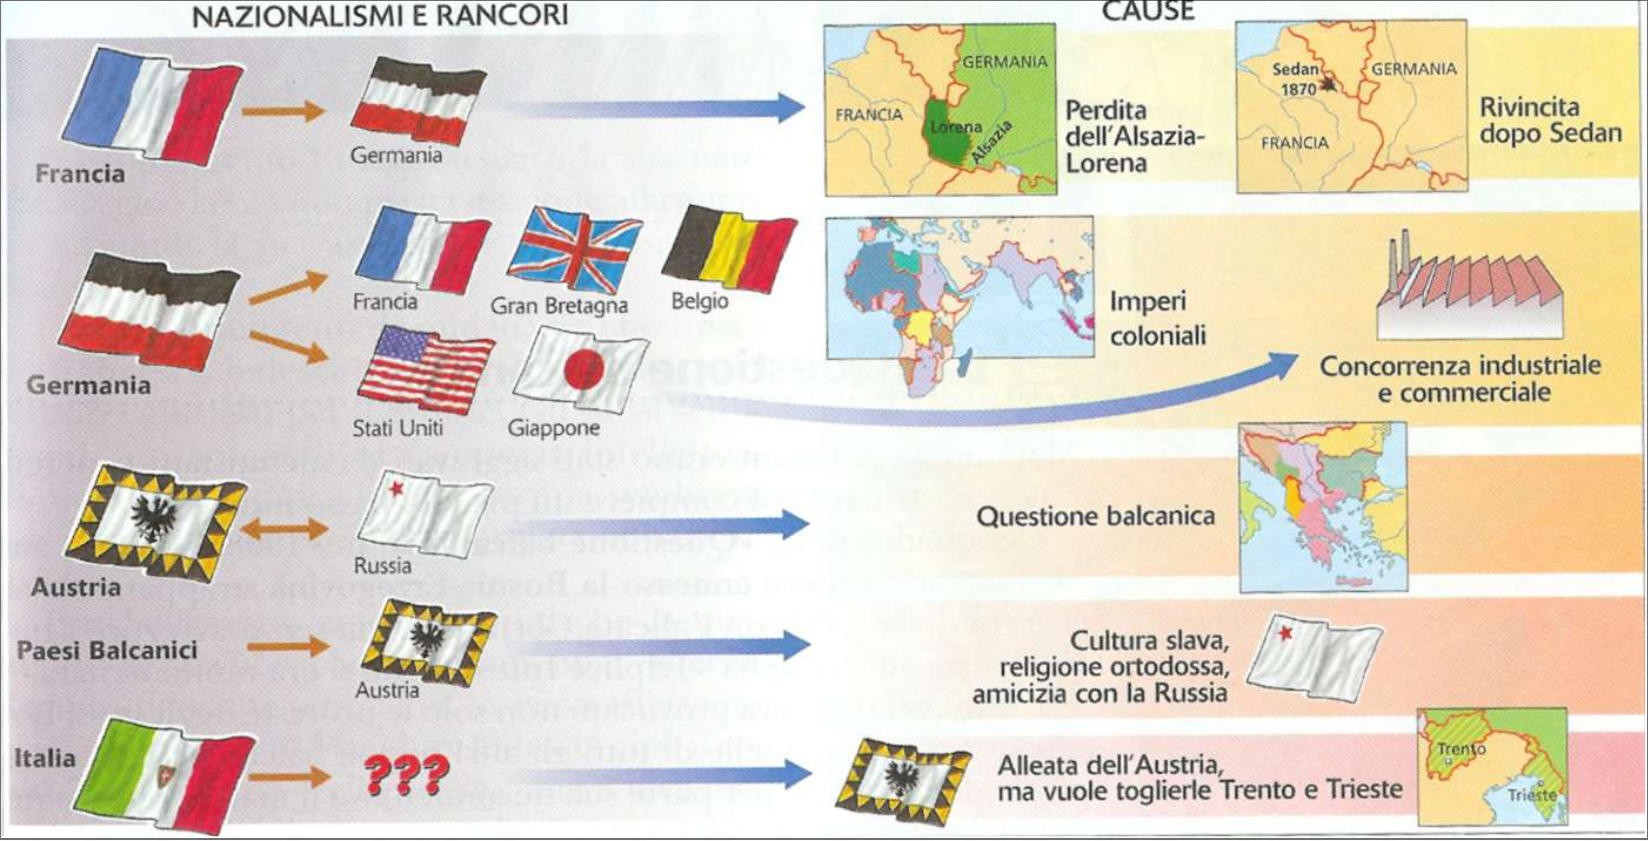
\includegraphics[width=0.95\textwidth]{./resources/europa_1914.png}
        \caption{Europa nel 1914}
    \end{figure}
    \end{center}
\end{snippet}

\begin{snippet}{tensioni-europa-1914}
    Nel 1914 vi sono diverse tensioni in Europa:
    \begin{itemize}
        \item \textbf{rivalità imperialistiche:} Le grandi potenze europee competevano per il controllo delle colonie e delle risorse in tutto il mondo, portando a conflitti di interessi e scontri diplomatici;
        \item \textbf{competizione economica:} L'industrializzazione accelerata aveva portato a una crescente competizione economica tra le nazioni europee per mercati, risorse e investimenti;
        \item \textbf{alleanze militari:} Gli accordi di alleanza, come la Triplice Intesa tra Francia, Russia e Regno Unito, e la Triplice Alleanza tra Germania, Austria-Ungheria e Italia, hanno creato un'atmosfera di tensione e incertezza, in cui un conflitto tra due stati poteva facilmente coinvolgere tutti gli altri;
        \item \textbf{nazionalismo:} Il nazionalismo sfrenato ha alimentato sentimenti di superiorità e rivalità tra le nazioni, portando a tensioni etniche e territoriali, specialmente nei Balcani;
        \item \textbf{crisi nei Balcani:} La regione balcanica era un crogiolo di tensioni etniche e nazionalistiche, con l'Impero Austro-Ungarico e la Russia che competevano per l'influenza, mentre stati emergenti come la Serbia cercavano l'indipendenza;
        \item \textbf{corsa agli armamenti:} Le potenze europee stavano investendo massicciamente nella costruzione di eserciti e flotte, alimentando una corsa agli armamenti che aumentava la tensione e il timore di un conflitto imminente;
        %Crisi diplomatiche: Una serie di crisi diplomatiche, come la Crisi di Agadir nel 1911 e la Crisi di Bosnia nel 1908-1909, avevano già aumentato le tensioni tra le potenze europee, preparando il terreno per un conflitto su vasta scala.
    \end{itemize}
\end{snippet}

\section{Assassinio di Sarajevo}

\begin{snippet}{assassinio-sarajevo-expl}
    L'assassinio di Sarajevo è avvenuto il 28 giugno 1914
    quando l'arciduca austro-ungarico Francesco Ferdinando e
    sua moglie Sofia sono stati assassinati a Sarajevo,
    Bosnia ed Erzegovina, da Gavrilo Princip,
    un nazionalista serbo-bosniaco.
    Questo evento ha innescato una serie di eventi che hanno portato alla
    scoppio della prima guerra mondiale.

    Questo evento è spesso considerato come la goccia che fece traboccare il vaso
    per ciò che concerne la Prima Guerra Mondiale.
\end{snippet}

\section{Sistema di alleanze}

\begin{snippetdefinition}{lega-dei-tre-imperatori-definizione}{Lega dei tre imperatori}
    L'\textit{alleanza dei tre imperatori}
    fu un accordo politico concluso nel
    1873 fra Guglielmo I di Germania, Francesco Giuseppe d'Austria e Alessandro II di Russia.
\end{snippetdefinition}

\plain{l trattato stabiliva la concertazione fra Austria e Russia in caso
di crisi internazionale e l'impegno a risolvere pacificamente eventuali dispute.}

\begin{snippetdefinition}{alleanza-austro-tedesca-definizione}{Duplice alleanza con Austria}
    La \textit{Duplice alleanza} (\textit{Alleanza austro-tedesca})
    del 1879 fu un patto militare difensivo firmato nel 1879 a Vienna da Germania
    e Austria-Ungheria, motivato dal pericolo di un attacco della Russia ad una delle due potenze.
\end{snippetdefinition}

\begin{snippetdefinition}{triplice-alleanza-definizione}{Triplice allenaza}
    La \textit{Triplice alleanza} (1882)
    fu un patto militare difensivo stipulato il 20 maggio 1882 a
    Vienna dagli imperi di Germania e Austria-Ungheria
    (che già formavano la Duplice alleanza) e dal Regno d'Italia. 
\end{snippetdefinition}

\begin{snippet}{f3bb73aa-c8be-4bb2-8e9b-3f0c5daabfbd}
    La Duplice alleanza diventa quindi la Triplice alleanza 
    con l'entrata dell'Italia.
    
    % V. Berghahn - La formazione dei due sistemi di alleanze
    
    Vedendo che la Germania ricorre alle armi, alimentando la corsa agli armamenti, la Gran Bretagna
    decise di uscire dal suo \quotes{splendido isolamento}, ossia dalla sua posizione di balancer delle
    posizione europee.
    
    L'Inghilterra, in risposta alla Weltpolitik tedesca e ai suoi
    piani di riarmo navale, ha abbandonato il suo isolamento politico,
    stringendo alleanze con il Giappone e la Francia.
    Queste mosse hanno portato alla formazione della Triplice Intesa,
    contrapposta all'alleanza tra Germania,
    Austria-Ungheria e Italia.
    Le tensioni si sono accentuate con la crisi marocchina del 1905 e
    gli accordi russo-britannici del 1907, mentre la corsa agli armamenti e
    la propaganda nazionalista hanno alimentato il clima di conflitto.
\end{snippet}

\begin{snippetdefinition}{duplice-intesa-definizione}{Duplica intesa}
    La \textit{Duplice intesa}
    fu un patto militare difensivo tra la Francia e la Russia definitosi fra il 1891 e il 1894 in tre fasi.
\end{snippetdefinition}

\begin{snippet}{c06a325f-a4ce-4d61-9161-bd655b1f1cb4}
    Fu una risposta al rinnovo della Triplice alleanza tra Germania,
    Austria e Italia, nonché, stante la neutralità della Gran Bretagna,
    un tentativo di formare un equilibrio strategico in Europa.
\end{snippet}

\begin{snippetdefinition}{intesa-cordiale-definizione}{Intesa cordiale}
    L'\textit{Intesa cordiale}
    fu un accordo stipulato l'8 aprile 1904 tra Francia
    e Gran Bretagna per il reciproco riconoscimento di sfere d'influenza coloniale. 
\end{snippetdefinition}

\begin{snippetdefinition}{triplice-intesa-definizione}{Triplice intesa}
    La \textit{Triplice intesa}
    fu un sistema di accordi politico-militari tra il Regno Unito,
    la Francia e la Russia culminato nell'accordo anglo-russo del 1907.
\end{snippetdefinition}

\begin{snippet}{7adff7f1-1f1b-4e44-82d4-2d1ef2db8526}
    La Triplice intesa si oppose alla Triplice alleanza.

    Queste alleanze delineano quindi due blocchi che rimarranno fino allo scoppio della Prima
    Guerra Mondiale.
    
    % IRRIDENTISMO -- da qualche parte
\end{snippet}

\section{La guerra}

\begin{snippet}{b0fe1173-8c13-4923-a689-fa1dd2ff62c3}
    La Prima Guerra Mondiale sarebbe dovuta essere una guerra lampo, ma diventò la prima
    vera guerra di logoramento.
    
    I giovani (della generazione del 1914) che si arruolano con fervore
    all'inizio della prima guerra mondiale.
    Il loro entusiasmo era plasmato dalle innovazioni tecnologiche e culturali del tempo,
    incarnate dai movimenti futuristi ed espressionisti che esaltavano velocità,
    violenza e conflitto.
    La guerra rappresentava per molti di loro un'opportunità di liberazione sociale e
    di espressione individuale ei di virilità.
    Era vista come il mezzo per abbattere l'ipocrisia e la tirannia borghese,
    dando vita a un nuovo ordine sociale e sottolineando il proprio patriottismo.
\end{snippet}

\begin{snippetdefinition}{futurismo-definizione}{Futurismo}
    Il \textit{futurismo} è un movimento culturale che nasce in Italia nel
    1909. Secondo il futurismo la velocità è la misura di tutte le cose.
\end{snippetdefinition}

\begin{snippetdefinition}{irredentismo-definizione}{Irredentismo}
    L'\textit{irredentismo} è una politica o un movimento che 
    mira a recuperare territori storicamente appartenuti a un determinato stato,
    ma che sono stati persi a seguito di eventi come guerre o trattati internazionali.
\end{snippetdefinition}

\begin{snippet}{c0583405-3284-4d41-a8a6-cbdb8690f8c3}
    Solitamente, questo concetto è associato alla volontà di riunificare territori
    abitati da persone con una comune identità culturale, linguistica o etnica.
    Ad esempio, l'irredentismo italiano durante il XIX e il XX secolo mirava a
    riunire territori abitati da italiani, come il Trentino e l'Istria, che erano
    sotto il controllo di altri stati.

    % documento la posta in gioco
\end{snippet}

\begin{snippet}{ccb22560-1144-44d1-857f-fee9dab820ff}
    \begin{chronology}[10]{1870}{1920}{\textwidth}
        \event{1873}{(1873) Patto dei 3 Imperatori}
        \event{1879}{(1879) Duplice Alleanza Ger-A-U}
        \event{1882}{(1882) Triplice alleanza Ger-AU-I}
        \event{1904}{(1904) Intesa cordiale Italia-Inghilterra}
        \event{1905}{(1905) Crisi marocchina}
        \event{1907}{(1907) Triplice Intesa Fr-Ingh-Russia}
        \event{1909}{(1909) Primo manifesto futurista}
        \event{1914}{(1914) Germania attacca la Francia} % passando dal Belgio neutrale
        
        \event[1890]{1920}{} % Corsi agli armamenti
    \end{chronology}
    {\color{gray} (1890-1920) Corsa agli armamenti}
\end{snippet}

\begin{snippetdefinition}{trincea-definizione}{Trincea}
    La \textit{trincea} è un tipo di fortificazione militare difensiva
    costituita, nella sua forma più semplice, da un
    fossato lineare scavato nel terreno per ospitare al suo interno le
    truppe, che in questo modo si trovano protette dal tiro delle armi nemiche.
\end{snippetdefinition}

\begin{snippetdefinition}{piano-schlieffen-definizione}{Piano Schlieffen}
    Il \textit{Piano Schlieffen} fu un piano strategico dello Stato Maggiore
    tedesco, concepito nel 1905 in previsione di una
    guerra su due fronti (ad est contro la Russia e ad
    ovest contro la Francia e il Regno Unito),
    guerra che la Germania temeva di dover prima o poi
    affrontare in seguito all'alleanza tra Francia e Russia e
    all'accordo stipulato con la Entente cordiale tra Francia e
    Gran Bretagna. Il piano prese il nome dal suo autore, il capo di Stato Maggiore Alfred Graf von Schlieffen. 
\end{snippetdefinition}

% Cartina con le freccie Piano Schlieffen

\begin{snippet}{04920c78-8c84-43d0-a1ed-8756003d09cd}
    Alcuni dei difetti che portarono al fallimento del Piano non sono
    a posteriori addebitabili al solo von Moltke,
    bensì erano connaturati al piano stesso, che sottovalutava in generale gli
    avversari, dal piccolo Belgio alla grande Russia.
\end{snippet}

\begin{snippetdefinition}{battaglie-ypres-definizione}{Battaglie di Ypres}
    Le \textit{battaglie di Ypres} consistono in cinque
    combattimenti vicino alla città belga di Ypres fra la Germania
    e Francia, Regno Unito e Belgio.
\end{snippetdefinition}

\begin{snippet}{6b71dc99-e2bf-46f5-9038-68c0eb31c6dc}
    La seconda battaglia di Ypres (1915) fu il primo conflitto ad impiegare
    un attacco massiccio con gas nocivo.
    
    % Testo:
    % Scemi di guerra. La follia nelle trincee
    
    Il ruolo dello stato diventa sempre più presente
    all'interno della vita pubblica e diventa uno dei primi investitori
    nelle nuove tecnologie, colui che commissione alle industrie (soprattutto quella bellica)
    la produzione.
    Lo stato investe anche nella propaganda.
    
    \textbf{Guerra moderna:} \\
    Modernità rappresentata dalle nuove armi con nuova potenza di fuoco
    (lanciafiamme, mitra, armi chimiche, mezzi corazzati)
    \(\rightarrow\) Eserciti imponenti e meglio armati (fucili a ripetizione, cannoni, mitragliatrici automatiche, ...).
    
    Vi sono diverse manifestazioni come rifiuto della guerra (diserzione e autolesionismo).
\end{snippet}

\begin{snippetdefinition}{shell-shock-definizione}{Shell shock}
    La \textit{nevrosi di guerra} o \textit{shell shock}
    è un termine che ha avuto origine durante la prima
    guerra mondiale per descrivere il tipo di disturbo da stress
    post-traumatico (PTSD) che molti soldati sperimentarono durante la guerra.
\end{snippetdefinition}

\begin{snippet}{e1ee1ff9-4061-4238-bb8a-beaedfacb0d8}
    % i manifesti della propaganza, zio sam. vabbè.

    L'anno si svolta della prima guerra mondiale è il 1917 poiché
    gli Stati Uniti entrano a far parte del conflitto contro la Germiania (guerra sottomarina)
    e per via della rivoluzione russa (rovesciamento dello zar).
\end{snippet}

\section{I 14 punti di Wilson}

\begin{snippet}{b41f6649-5556-45ca-9152-0f50a27f87d9}
    All'indomani della Prima guerra mondiale quattro imperi (tedesco, austro-ungarico, russo e
    ottomano) erano scomparsi e, con l'emergere degli Stati Uniti a grande potenza internazionale,
    un'Europa devastata dalla guerra aveva cessato di essere il centro del mondo. Insieme ai vecchi
    ordinamenti, anche un universo di valori e tradizioni era stato spazzato via. Il conflitto non si
    risolse solo in un azzeramento dell'assetto precedente, ma genero e alimento le aspirazioni
    verso una societa nuova, piu libera e giusta. Tornata la pace, il presidente americano Thomas
    Woodrow Wilson propose di ridefinire i rapporti internazionali e di porre fine alla vecchia
    logica imperialistica.
    
    Già nel gennaio del 1918, quando la sconfitta degli Imperi centrali sembrava imminente, il
    presidente americano Wilson aveva illustrato al Congresso un programma in 14 punti, in cui
    enunciava i principi su cui costruire una pace giusta e duratura. Di fronte alle distruzioni e agli
    sconvolgimenti provocati dalle mire espansionistiche delle potenze europee, Wilson proponeva
    un nuovo sistema di relazioni internazionali fondato sulla cooperazione fra stati,
    sull'emancipazione delle nazionalita oppresse e sul riconoscimento dei "diritti inviolabili dei
    popoli dell'umanita".
    
    % i 14 punti
\end{snippet}

\section{Trattati di pace}

\begin{snippetdefinition}{conferenza-pace-parigi-definizione}{Conferenza di pace di Parigi}
    La \textit{conferenza di pace di Parigi} del 1919 fu una conferenza di
    pace organizzata dai paesi usciti vincitori dalla prima guerra mondiale,
    impegnati a delineare una nuova situazione geopolitica in Europa e a
    stilare i trattati di pace con le potenze centrali uscite sconfitte dalla guerra. 
\end{snippetdefinition}

\plain{Vengono istituiti dei trattati di pace separati:}

% - Con la Germania (trattato di Versailles 1919);
%- Con l’Austria-Ungheria (trattato di Saint-German-en-Laye, settembre 1919);
%- Con la Bulgaria (trattato del Trianon, giugno 1920);
%- Con la Turchia (trattato di Sevres, agosto 1920)

\begin{snippetdefinition}{trattato-sevres-turchia-definizione}{Trattato di Sèvres con la Turchia}
    Il \textit{trattato di Sèvres} è stato il trattato di pace firmato
    tra le potenze alleate della prima guerra mondiale e l'Impero ottomano il
    10 agosto 1920 presso la città francese di Sèvres.
\end{snippetdefinition}

\begin{snippetdefinition}{trattato-versailles-definizione}{rattato di Versailles}
    Il \textit{trattato di Versailles} fu stipulato nell'ambito
    della conferenza di pace di Parigi del 1919 e firmato da 44
    Stati il 28 giugno 1919 a Versailles.
\end{snippetdefinition}

\begin{snippet}{6af9a5f5-9e95-488b-b2b4-c50e6b40cfd2}
    Durante la discussione sul primo trattato di pace, quello con la Germania, apparve subito
    evidente quanto le posizioni di Francia e Gran Bretagna fossero distanti dal programma di
    Wilson. I rappresentanti francesi manifestarono infatti una risoluta volonta punitiva nei
    confronti della Germania: quattro anni di invasione e di battaglie durissime avevano esacerbato
    l'odio antitedesco e ora la Francia era decisa a condannare la Germania a una condizione
    definitiva di irreversibile di inferiorita.
    La Gran Bretagna appoggio le pretese di Parigi perche contava di ottenere in cambio dei
    vantaggi nella parallela trattativa per la spartizione del Medio Oriente, regione ricca di petrolio,
    una risorsa divenuta di enorme importanza strategica con la motorizzazione degli eserciti e dei
    trasporti marittimi. Il solo Wilson cerco di moderare, almeno in parte, le pretese francesi. Il
    trattato di Versailles attribuì dunque allo Stato tedesco l'unica responsabilita e l'intera "colpa"
    del conflitto. La "pace punitiva" impose alla Germania una serie di durissime condizioni (il
    cosiddetto Diktat):
    \begin{enumerate}
        \item La cessione di tutte le colonie tedesche, che vennero spartite soprattutto tra Parigi e
        Londra;
        \item La restituzione dell'Alsazia e della Lorena alla Francia;
        \item La cessione, per quindici anni, del ricco bacino carbonifero della Saar al governo
        francese;
        \item La restituzione dello Schleswig alla Danimarca.
    \end{enumerate}
    Inoltre alcune regioni orientali (l'Alta Slesia e la Posnania) andarono al ricostituito Stato della
    Polonia; a questi si aggiungeva il "corridoio di Danzica" (o "corridoio polacco"), una striscia di
    terra che assicurava alla Polonia uno sbocco sul mar Baltico e separava la Prussia orientale dal
    resto della Germania.
    In totale, circa due milioni di tedeschi si trovarono da un giorno all'altro espulsi dai confini
    nazionali.
    
    Le clausole militari del trattato imposero alla Germania:
    \begin{itemize}
        \item Il sostanziale azzeramento della flotta e dell'aeronautica militare:
        \item L'abolizione della leva obbligatoria;
        \item La riduzione dell'esercito a soli 100.000 uomini dotati di armamenti leggeri;
        \item La smilitarizzazione di una fascia di 50 km sulla riva destra del Reno;
        \item L'occupazione per quindici anni della riva sinistra da parte di truppe francesi, belghe e inglesi.
    \end{itemize}
    
    In tal modo si intendeva infliggere un colpo definitivo al militarismo tedesco, per neutralizzarne
    qualsiasi velleita di potenza.
    
    Furono infine addebitati al governo di Berlino tutti i danni di guerra arrecati ai paesi vincitori.
    Di qui l'eccezionale entita delle riparazioni, fissate nel 1921 in 132 miliardi di marchi-oro da
    pagare in trent'anni: una somma enorme, che, nelle intenzioni dei vincitori, doveva impedire
    per lungo tempo qualsiasi possibilita di ripresa dell'economia tedesca. Esclusi dalle trattative, i
    diplomatici tedeschi poterono solo controfirmare il trattato (28 giugno 1919).
\end{snippet}

\begin{snippetdefinition}{trattato-saint-germain-en-laye-definizione}{Trattato di Saint-Germain-en-Laye}
    Il trattato di Saint-Germain-en-Laye
    stabilisce la ripartizione del dissolto Impero austro-ungarico
    e le condizioni per la creazione della Repubblica austriaca. 
\end{snippetdefinition}

\begin{snippetdefinition}{trattano-trianon-definizione}{Trattato di Trianon}
    Il \textit{trattato del Trianon} stabilisce la sorte
    del Regno d'Ungheria in seguito alla dissoluzione dell'Impero austro-ungarico. 
\end{snippetdefinition}

% La nascita della Turchia conteporanea

\begin{snippetdefinition}{interventismo-definizione}{Interventismo}
    Con il termine \textit{interventismo} si intende,
    le posizioni assunte da alcune correnti politiche e di pensiero
    favorevoli all'intervento nella prima guerra mondiale.
\end{snippetdefinition}

\plain{Gli interventisti si oppongono ai <b>neutralisti</b>.}

\begin{snippetdefinition}{patto-londra-definizione}{Patto di Londra}
    Il \textit{Patto di Londra} fu un accordo segreto firmato il
    26 aprile 1915, stipulato tra il governo italiano
    (nonostante già impegnato nella Triplice alleanza,
    il patto militare stipulato nel 1882 da Germania,
    Austria-Ungheria e Italia) e i rappresentanti della Triplice Intesa,
    con i quali l'Italia si impegnò a scendere in guerra contro gli Imperi centrali
    durante la prima guerra mondiale. 
\end{snippetdefinition}

\begin{snippetdefinition}{societa-delle-nazioni-definizione}{La società delle nazioni}
    La \textit{Società delle Nazioni} (1919)
    stata la prima organizzazione intergovernativa
    avente come scopo quello di accrescere il benessere
    e la qualità della vita degli esseri umani.
    Il suo principale impegno
    era quello di prevenire le guerre,
    sia attraverso la gestione diplomatica dei conflitti
    sia attraverso il controllo degli armamenti; 
\end{snippetdefinition}

\begin{snippet}{9710d3a9-35d0-45d9-ac55-9092fd528fd7}
    Con il trattato di Versailles entrò in vigore anche il patto costitutivo della Società delle Nazioni.
    Questo organismo sovranazionale, fortemente voluto dal presidente americano Wilson, aveva
    sede a Ginevra e si componeva di:
    \begin{itemize}
        \item un'Assemblea, alla quale partecipavano su un piano di parità tutti i paesi aderenti;
        \item un Consiglio di 9 membri, di cui 5 permanenti (Gran Bretagna, Francia, Stati Uniti, Italia
            e Giappone) e 4 eletti dall'Assemblea; su qualsiasi questione, il Consiglio avrebbe dovuto
            deliberare all'unanimità.
    \end{itemize}
    
    La Società delle Nazioni aveva per suo compito fondamentale quello di garantire l'indipendenza
    e la sovranità di tutti gli stati membri (art. 10); in caso di contrasti internazionali, si sarebbe
    fatto ricorso alla mediazione e all'arbitrato (art. 13); se uno dei paesi avesse dichiarato guerra
    prima dello scadere di tre mesi dal tentativo di arbitrato, sarebbe stato messo al bando dalla
    Società e sarebbero scattate a suo carico adeguate sanzioni economiche (art. 16).
    Il fatto che ogni decisione dovesse essere assunta all'unanimità, come anche la mancanza di una
    forza militare e dunque di uno strumento in grado di imporre le decisioni prese e di far
    rispettare le eventuali sanzioni, si rivelarono negli anni successivi un limite che rese in pratica
    nulla la capacità operativa del nuovo organismo.
    
    La Società delle Nazioni si trovò inoltre subito gravemente indebolita dalla mancata adesione
    degli Stati Uniti: nel 1920 la nuova maggioranza repubblicana scelse di tornare all'
    isolazionismo, voltando le spalle ai principi wilsoniani.
\end{snippet}

\section{Conseguenze a lungo termine}

\begin{snippet}{2bcb028b-1bb5-4e7b-96c8-45870e30a284}
    \begin{itemize}
        \item grosse perdite di uomini, sia militari che civili;
        \item grandi distruzioni: costo della guerra molto alto e si somma al logorio
            degli impianti industriali; si ferma il progresso economico;
        \item indebitamento dei paesi belligeranti (debiti con USA);
        \item ristagno economico e alto tasso di disoccupazione; problema dei reduci;
        \item paesi occidentali cambiano i loro fornitori: non più are danubiana
            e Rhur, ma USA, Canada e Argentina;
        \item USA e Giappone principali beneficiari del cambiamento
            commerciale, le loro industrie suppliscono alla mancanza di prodotti europei;
        \item trattati di pace non risolvono i problemi che hanno generato la guerra;
        \item classi dirigenti incapaci di risolvere i problemi e i cambiamenti,
            a livello sociale tutte le classi sono socntente;
        \item malessere del proletariato urbano porta al Biennio rosso (1918-1920);
    \end{itemize}
\end{snippet}

\begin{snippetdefinition}{biennio-rosso-definizione}{Biennio Rosso}
    Il \textit{biennio rosso} 
    è stato un periodo
    della storia d'Italia compreso fra il
    1919 e il 1920, caratterizzato da una serie
    di lotte operaie e contadine che ebbero il
    loro culmine e la loro conclusione con
    l'occupazione delle fabbriche nel settembre 1920.
\end{snippetdefinition}

\begin{snippet}{1785be37-353c-45bd-bc25-e101f0262328}
    Il biennio rosso viene alimentato anche da ciò che sta accadendo in russia.

    Con la prima guerra mondiale le donne lavorano nella fabbricazione di materiale bellico e 
    specialmente munizioni.
\end{snippet}

\end{document}